\documentclass[hidelinks,12pt]{article}
\usepackage[utf8]{inputenc}
\usepackage[table,xcdraw]{xcolor}
\usepackage{mathtools}
\usepackage{amsthm}
\usepackage{amsmath}
\usepackage{amsfonts}
\usepackage{amssymb}
\usepackage{centernot}
\usepackage{marvosym}
\usepackage{enumitem}
\usepackage{hyperref}
\begin{document}
\graphicspath{{/home/theo/Documents/GitHub/Math-Homeworks/Math 531/Random/}}
\setcounter{tocdepth}{1}
\let\marvosymLightning\Lightning
\newtheorem{theorem}{Theorem}
\newtheorem{corollary}{Corollary}[theorem]
\newtheorem*{remark}{Remark}
\renewcommand\qedsymbol{QED}
\newcommand{\N}{\mathbb{N}}
\newcommand{\Z}{\mathbb{Z}}
\newcommand{\divby}{%
  \mathrel{\text{\vbox{\baselineskip.65ex\lineskiplimit0pt\hbox{.}\hbox{.}\hbox{.}}}}%
  }
\newcommand{\notdivby}{\centernot\divby}
\title{\scalebox{2}{Math 531 Homework 1}}
\author{\scalebox{1.5}{Theo Koss}}
\date{January 2021}
\maketitle
\section{Section 1.1}
\begin{itemize}
    \item Problem 1, Let $m,n,r,s\in\Z$. If $m^2+n^2=r^2+s^2=mr+ns$, prove that $m=r$ and $n=s$.
    \begin{proof}
    Assume, to the contrary, that $m\neq r$ and $n\neq s$. Then it follows that $m=r+a$ and $n=s+b$, for some $a,b\neq0\in\Z$. Then,\begin{equation}\label{eq1}
        m^2+n^2=(r+a)^2+(s+b)^2=r^2+2ra+a^2+s^2+2sb+b^2
    \end{equation}Also,\begin{equation}\label{eq2}
        mr+ns=r^2+ra+s^2+sb
    \end{equation}And since $r^2+s^2=mr+ns$, we deduce that\begin{equation}\label{eq3}
        r^2+ra+s^2+sb=r^2+s^2\implies ra+sb=0
    \end{equation}
    Since \ref{eq1} and \ref{eq2} are equal, we can set them equal and cancel terms, therefore:\begin{equation}\label{eq4}
        r^2+2ra+a^2+s^2+2sb+b^2=r^2+ra+s^2+sb\implies a^2+b^2+ra+sb=0
    \end{equation}
    By \ref{eq3}, $ra+sb=0$, so $$a^2+b^2=0$$\scalebox{1.5}{\Lightning}
    \end{proof}
    \item Problem 2, List all the numbers between 6 and the next perfect number, including divisors and sums of those divisors.
% Please add the following required packages to your document preamble:
% \usepackage[table,xcdraw]{xcolor}
% If you use beamer only pass "xcolor=table" option, i.e. \documentclass[xcolor=table]{beamer}
\begin{table}[h]
\begin{tabular}{|l|l|l|l|l|l|l|l|}
\hline
\rowcolor[HTML]{CBCEFB} 
Numbers                           & 7                            & 8                                         & 9                              & 10                                & 11                               & 12                                    & 13       \\ \hline
\rowcolor[HTML]{9AFF99} 
Divisors                          & 1,7                          & 1,2,4,8                                   & 1,3,9                          & 1,2,5,10                          & 1,11                             & 1,2,3,4,6,12                          & 1,13     \\ \hline
\rowcolor[HTML]{FFCE93} 
Sum of divisors                   & 1                            & 7                                         & 4                              & 8                                 & 1                                & 16                                    & 1        \\ \hline
\rowcolor[HTML]{CBCEFB} 
14                                & 15                           & 16                                        & 17                             & 18                                & 19                               & 20                                    & 21       \\ \hline
\rowcolor[HTML]{34FF34} 
1,2,7,14                          & 1,3,5,15                     & 1,2,4,8,16                                & 1,17                           & 1,2,3,6,9,18                      & 1,19                             & 1,2,4,5,10,20                         & 1,3,7,21 \\ \hline
\rowcolor[HTML]{FFCE93} 
10                                & 9                            & 15                                        & 1                              & 21                                & 1                                & 22                                    & 11       \\ \hline
\cellcolor[HTML]{CBCEFB}22        & \cellcolor[HTML]{CBCEFB}23   & \cellcolor[HTML]{CBCEFB}24                & \cellcolor[HTML]{CBCEFB}25     & \cellcolor[HTML]{CBCEFB}26        & \cellcolor[HTML]{CBCEFB}27       & \cellcolor[HTML]{CBCEFB}28            &          \\ \hline
\cellcolor[HTML]{67FD9A}1,2,11,22 & \cellcolor[HTML]{67FD9A}1,23 & \cellcolor[HTML]{67FD9A}1,2,3,4,6,8,12,24 & \cellcolor[HTML]{67FD9A}1,5,25 & \cellcolor[HTML]{67FD9A}1,2,13,26 & \cellcolor[HTML]{67FD9A}1,3,9,27 & \cellcolor[HTML]{67FD9A}1,2,4,7,14,28 &          \\ \hline
\cellcolor[HTML]{FFCE93}14        & \cellcolor[HTML]{FFCE93}1    & \cellcolor[HTML]{FFCE93}36                & \cellcolor[HTML]{FFCE93}6      & \cellcolor[HTML]{FFCE93}16        & \cellcolor[HTML]{FFCE93}13       & \cellcolor[HTML]{FFCE93}28            &          \\ \hline
\end{tabular}
\end{table}
(Sorry, formatting is weird)
\newpage\item Problem 9, Let $a,b,c\in\Z$ such that $a+b+c=0$, show that if $n\in\Z$ divides two of the integers, it divides all three.
\begin{proof}
If $n|a$ and $n|b$, then $a=np$, and $b=nq$. Then $a+b+c=np+nq+c=0$. So $c=-n(p+q)$, therefore $c$ is some multiple of $n$, thus $n|c$.
\end{proof}
\item Problem 15, For what $n\in\Z^+$ is $\gcd(n,n+2)=2$. Conjecture: $n=2k,k\in\N$.
\begin{proof}
Suppose $n=2k,k\in\N$, ($n$ is even). Then $$\gcd(n,n+2)=\gcd(2k,2k+2)=\gcd(2k,2)$$Since $2k$ is always even, $2|2k$, and 2 is the largest divisor because the largest number than can divide 2 is 2. Therefore $\gcd(n,n+2)=2$ when $n=2k$.
\end{proof}
\end{itemize}
\section{Section 1.2}
\begin{itemize}
    \item Problem 4, $\{1,7,11,13,17,19,23,29,31,37,41,43,47,49,53,59\}$. (For my work, sieved out all multiples of 2,3 and 5, this is what remained.)
    \item Problem 6, For each of 9,15,20,24,100, give a divisor diagram.\newline\scalebox{.2}{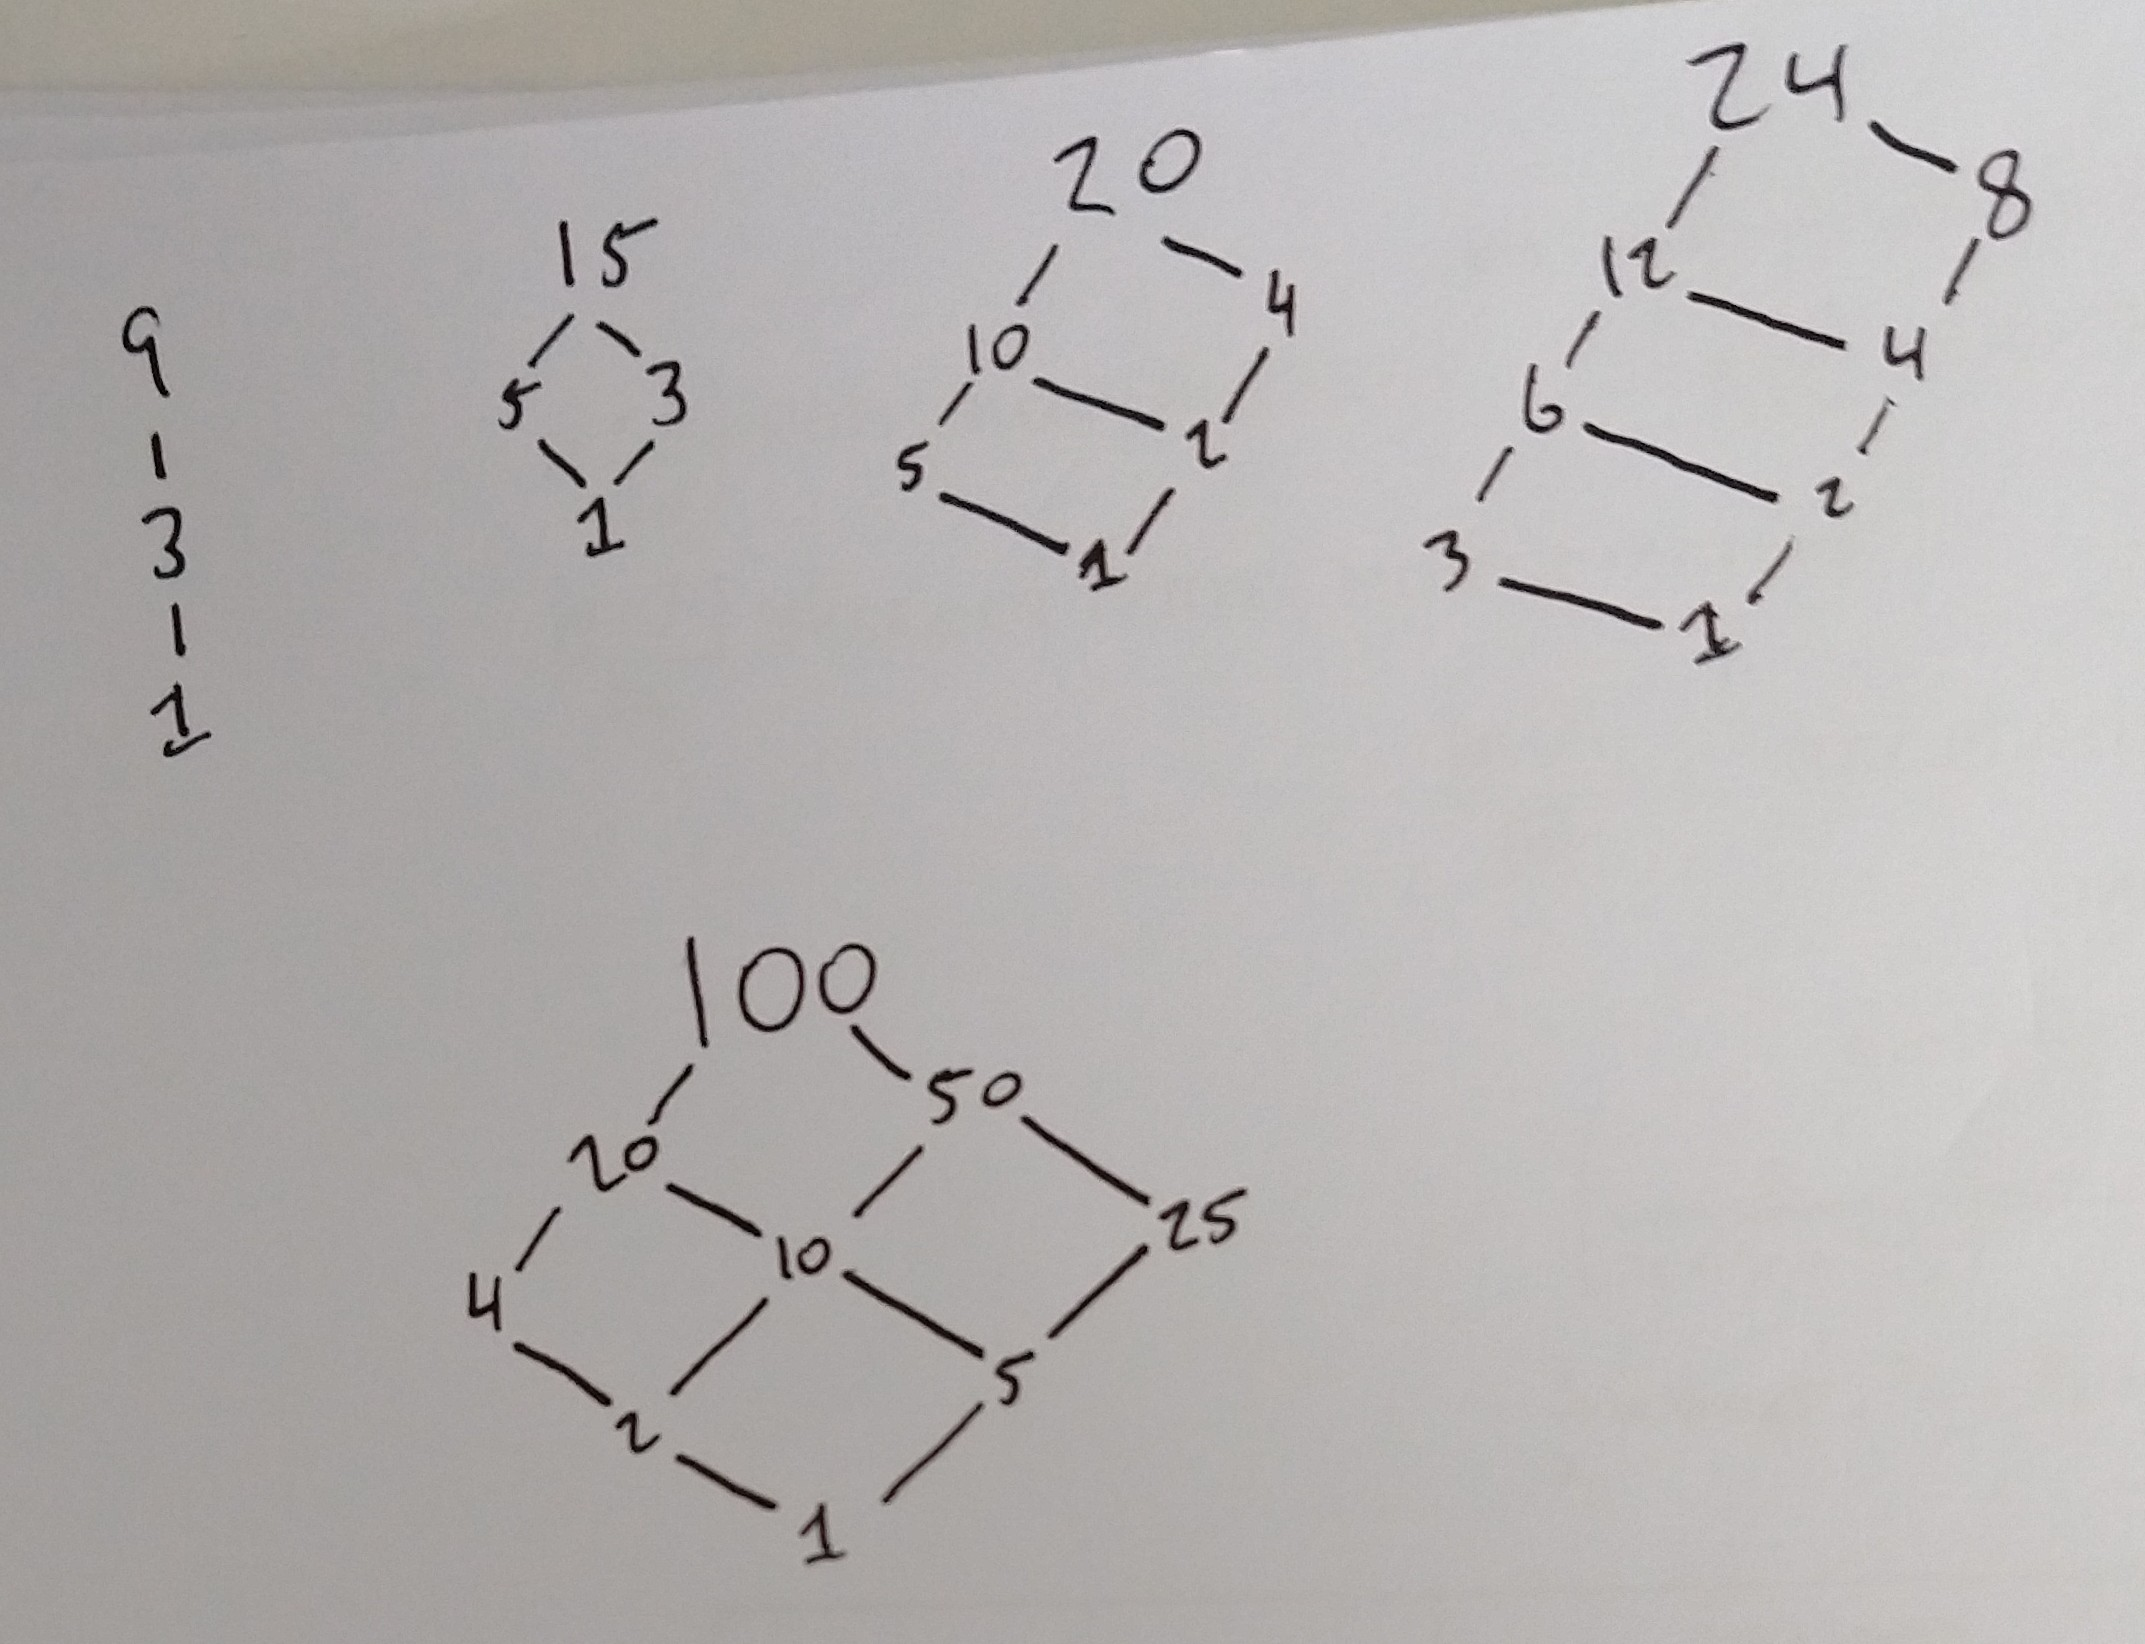
\includegraphics{DivisorDiagrams}}
    \item Problem 10, Prove that $n^4+4$ is composite if $n>1$.\begin{proof}
    $$n^4+4=(n^2-2n+2)(n^2+2n+2)$$And since $$(n^2-2n+2)\in\Z$$and $$(n^2+2n+2)\in\Z$$ and $$(n^2-2n+2)\neq(n^2+2n+2)$$ for $n>1\in\Z$, this is a product of two integers, therefore it is composite.
    \end{proof}
    \item Problem 24, Prove that every positive integer can be uniquely expressed as the product of a square and a square-free integer. (Kinda lost on this one but I'll give it a try)
    \begin{proof}
    By the FTA, every positive integer can be uniquely expressed as the product of primes, like so:$$a=(p_1^{n_1}p_2^{n_2}p_3^{n_3}...p_k^{n_k})=\prod_{i=1}^kp_i^{k_i}$$ (Ok I'm confused here, for example how is 6 created with a square? Does 1 count as a square? It must because there's no other way to get all the primes.) I was thinking about splitting $a$ into parts, one square part and one square-free part, like: $$a=\underbrace{(p_1^{n_1}p_2^{n_2}p_3^{n_3}...p_k^{n_k})^2}_{\text{Squares}}\cdot\underbrace{(q_1^{m_1}q_2^{m_2}q_3^{m_3}...q_l^{m_l})}_{\text{Square-frees}}$$But I'm not sure if that's mathematically rigorous.
    \end{proof}
\end{itemize}
\end{document}
